\section{Experiments \& Results} % 4
\label{sec:experiments}

\subsection{Experimental settings} % 4.1
\label{subsec:exp_settings}

\paragraph{Data Processing}
Our experimental setup aligns with established DAS benchmark splits \citep{das2010farfar} for compatibility with existing evaluation protocols \citep{joshi2025grnade}. We implement strict length consistency filtering to remove preference pairs where sequence lengths differ or do not match graph node counts, ensuring training stability and preventing spurious length-based correlations. Following preprocessing, our dataset comprises 20,811 training pairs, 505 validation pairs, and 429 test pairs, drawn from 4,025 training instances, 100 validation instances, and 98 test instances.  This testing dataset split has overlap with the training dataset of RiboDiffusion \citep{huang2024ribodiffusion} and RDesign \citep{tanrdesign}, which leads to the abnormally high sequence recovery (100\%) for some structures like 7D7W.

\paragraph{Evaluation Protocol and Metrics}
We evaluate all approaches, generating 8 sequence candidates under temperature $0.1$ per backbone for statistical reliability. We directly apply the SSTT evaluation pipeline (Section\ref{subsec:sstt}) with EternaFold \citep{waymentsteele2022eternafold} for secondary structure predictions, and RhoFold+ \citep{shen2024accurate} for tertiary structure prediction. Furthermore, we report thresholded success rates, including percentages achieving RMSD $\leq$ 15.0\AA, pLDDT $\geq$0.50, MFE $\leq$ -8.0 $kcal/mol$, and TM $\geq$ 0.05. 

We evaluated pass@k performance \citep{lyu2024passk,wu2025invisible} by sampling 64 sequences per RNA structure (folded by RhoFold+ ~\citep{shen2024accurate}) and measuring success rates across different k values (1, 2, 4, 8, 16, 32, 64). For a given structure and k value, pass@k is defined as:
\begin{equation}
\text{pass@k} \;=\; 1-(1-p)^k .
\end{equation}
where p denotes the indicator function, returning 1 when the case pass the criteria, and returning 0 otherwise. 


\paragraph{Baseline Approaches}
We compare RiboPO against recent deep learning based RNA inverse folding models spanning two main paradigms. 
\textbf{Autoregressive models} include gRNAde \citep{joshi2025grnade}, RDesign \citep{tanrdesign}, R3Design \citep{tan2025r3design}, RiFold \citep{liu2025sentences}, and RhoDesign \citep{wong2024deep}.
\textbf{Diffusion-based models} include RiboDiffusion \citep{huang2024ribodiffusion}, RhoDesign \citep{wong2024deep} and \textbf{RIdiffusion} \citep{Hou2025ridiffusion}.



\subsection{SSTT Benchmark Analysis}
\label{subsec:benchmark_analysis}

\textbf{Baseline overview.}
We evaluate all four SSTT dimensions comprehensively (Table~\ref{tab:main_results_full}). Among baselines, \textbf{gRNAde} delivers the strongest sequence- and secondary-structure metrics, reflecting its GNN–GVP backbone conditioning. \textbf{Single-round RiboPO improves secondary and thermodynamic properties.}
Our first-round DPO (\textbf{RiboPO Round 1}) shows that even a single training round markedly enhances secondary-structure and thermodynamic properties over the gRNAde base model. Despite a minor decline in recovery (0.5288 $\rightarrow$ 0.504), RiboPO increases diversity (0.83 $\rightarrow$ \textbf{0.90}) and improves scMCC (0.60 $\rightarrow$ 0.71) and MFE ($-32.83$ $\rightarrow$ \textbf{$-35.83$}). This indicates that policy optimization effectively trades off marginal sequence similarity for substantially better foldability and energetic favorability. This represents early-stage exploration of a broader biophysically plausible sequence with improved stability. \textbf{Progressive refinement through multiple rounds.}
As RiboPO proceeds to multiple rounds, \textbf{thermostability gains become striking}. By Round 2, MFE further improves to \textbf{$-36.86$ kcal/mol}, the best of all models, while scMCC remains high (0.70) and tertiary metrics (RMSD and \%RMSD$\leq$8Å) also improve. These gains demonstrate that decreasing $\gamma_r$ across rounds—our “coarse-to-fine” margin schedule—admits increasingly subtle yet energetically favorable sequences, allowing the model to internalize thermodynamic regularities and better capture RNA structure–stability trade-offs. \textbf{Balanced sequence and structural fidelity.}
Although RiboPO prioritizes stability and secondary structure, its tertiary metrics remain competitive. Across all rounds, pLDDT holds steady at $\sim$0.65, RMSD stays near 10.4Å, and TM-score remains comparable to or better than several baselines. This suggests that thermodynamic optimization does not compromise 3D fidelity; instead, multi-round training preserves global structure while refining local and energetic features. In RNA terms, the model learns not only to produce sequences that fold correctly but also to maintain a realistic conformational ensemble.

% 我觉得这个是一个很好的角度，说这个的时候同时分析其他baseline，其实也是存在这种trade-off的，我们可以说我们的构建ppair的方式能够更好balance这种trade-off，由于SFT loss以及regularization term in DPO loss。
% 要具体分析哪些升了哪些降了，结合我们的pair构建指标，看看有没有什么规律
\begin{table*}[ht!]
\centering
\caption{Main benchmark results on the DAS test set. RiboPO significantly outperforms baselines on thermostability and secondary structure metrics (T and S), while remaining competitive on sequence and tertiary structure metrics (S and T). Best results are in \textbf{bold}.}
\label{tab:main_results_full}
\resizebox{\textwidth}{!}{%
\begin{tabular}{lccccccccc}
\toprule
\multirow{2}{*}{\textbf{Model}} 
& \multicolumn{2}{c}{\cellcolor{blue!10}\textbf{S (Sequence)}} 
& \multicolumn{1}{c}{\cellcolor{blue!10}\textbf{S (2D Struct.)}} 
& \multicolumn{5}{c}{\cellcolor{blue!10}\textbf{T (3D Struct.)}} 
& \multicolumn{1}{c}{\cellcolor{blue!10}\textbf{T (Thermo.)}} \\
\cmidrule(lr){2-3} \cmidrule(lr){4-4} \cmidrule(lr){5-9} \cmidrule(lr){10-10}
& \makecell{Rec.\\($\uparrow$)} & \makecell{Div.\\($\uparrow$)} & \makecell{scMCC\\($\uparrow$)} & \makecell{pLDDT\\($\uparrow$)} & \makecell{\%pLDDT\\$\geq$0.70} & \makecell{RMSD\\($\downarrow$)} & \makecell{\%RMSD\\$\leq$8\AA} & \makecell{TM-sc.\\($\uparrow$)} & \makecell{MFE\\($\downarrow$)} \\
\midrule
RiFold & 0.416 & 0.89 & 0.28 & 0.50 & 0.012 & 17.06 & 0.20 & 0.12 & -11.34 \\
RDesign & 0.415 & 0.84 & 0.20 & 0.45 & 0.22 & 16.81 & 0.12 & 0.12 & -10.59 \\
% R3Design\textsuperscript{*} & 0.539 & 0.41 & 0.66 & 0.68 & 0.54 & 6.20 & 0.76 & 0.48 & -24.48 \\
% RiboDiffusion\textsuperscript{*} & 0.775 & 0.22 & 0.86 & 0.77 & 0.82 & 3.69 & 0.90 & 0.62 & -22.40 \\
% RhoDesign\textsuperscript{*} & 0.648 & 0.62 & 0.29 & 0.56 & 0.29 & 12.17 & 0.39 & 0.26 & -15.76 \\
RIDiffusion & \textbf{0.533} & 0.85 & 0.59 & 0.60 & 0.28 & 10.66 & 0.46 & 0.25 & -28.81 \\
gRNAde (Base) & 0.529 & 0.83 & 0.60 & 0.62 & 0.38 & 11.45 & 0.42 & 0.29 & -32.83 \\
\midrule
RiboPO (Round 1) & 0.504 & \textbf{0.90} & 0.71 & \textbf{0.66} & \textbf{0.45} & 10.40 & 0.45 & 0.30 & -35.83 \\
RiboPO (Round 2) & 0.502 & 0.88 & 0.70 & 0.65 & 0.45 & \textbf{10.23} & \textbf{0.51} & \textbf{0.31} &  \textbf{-36.86} \\
RiboPO (Round 4) &  0.506 &  0.89 &  \textbf{0.72} & 0.65 & 0.42 & 10.42 & 0.44 & 0.29 &  -35.22 \\   
% Note: original 2D EteraFold data: base 0.6063; MFE, +12.28%
\bottomrule
\end{tabular}%
}
\raggedright
% \textsuperscript{*}\footnotesize{Results should be interpreted with caution due to overlaps in testing datasets with our benchmark splits.}

\end{table*}



\subsection{Advanced Analysis of Reinforcement Learning Effects}

\paragraph{RiboPO improves hit rate and sampling efficiency.}
We assess sampling efficiency using pass@k analysis on the identified 14 important RNA structures by \citep{das2010farfar} (Table~\ref{tab:pass_at_k}). For small $k$ values (pass@1–4), RiboPO achieves 37\%-44\% relative increase in success rate. Even at large $k$ (pass@32–64) Figure~\ref{fig:passk_curve}, RiboPO sustains 11\% higher success rates. This demonstrates that DPO improves the “hit rate” of high-quality sequences per sampling budget, which is critical when each candidate must be computationally folded. From an RL perspective, this reflects curriculum-based refinement that concentrates probability mass in high-reward regions; from an RNA perspective, it means fewer trials are needed to find sequences satisfying structural and energetic constraints, thereby reducing in silico or wet-lab burden.
% 按照现有思路就行，先分析随着k增大，有没有被超过，再有就是分析增速。因为新结果多了multi-round，可以尝试找一下multi和single的区别

% % === Figure: Pass@k curves (main text) ===
% \begin{figure}[t]
%   \centering
%   % 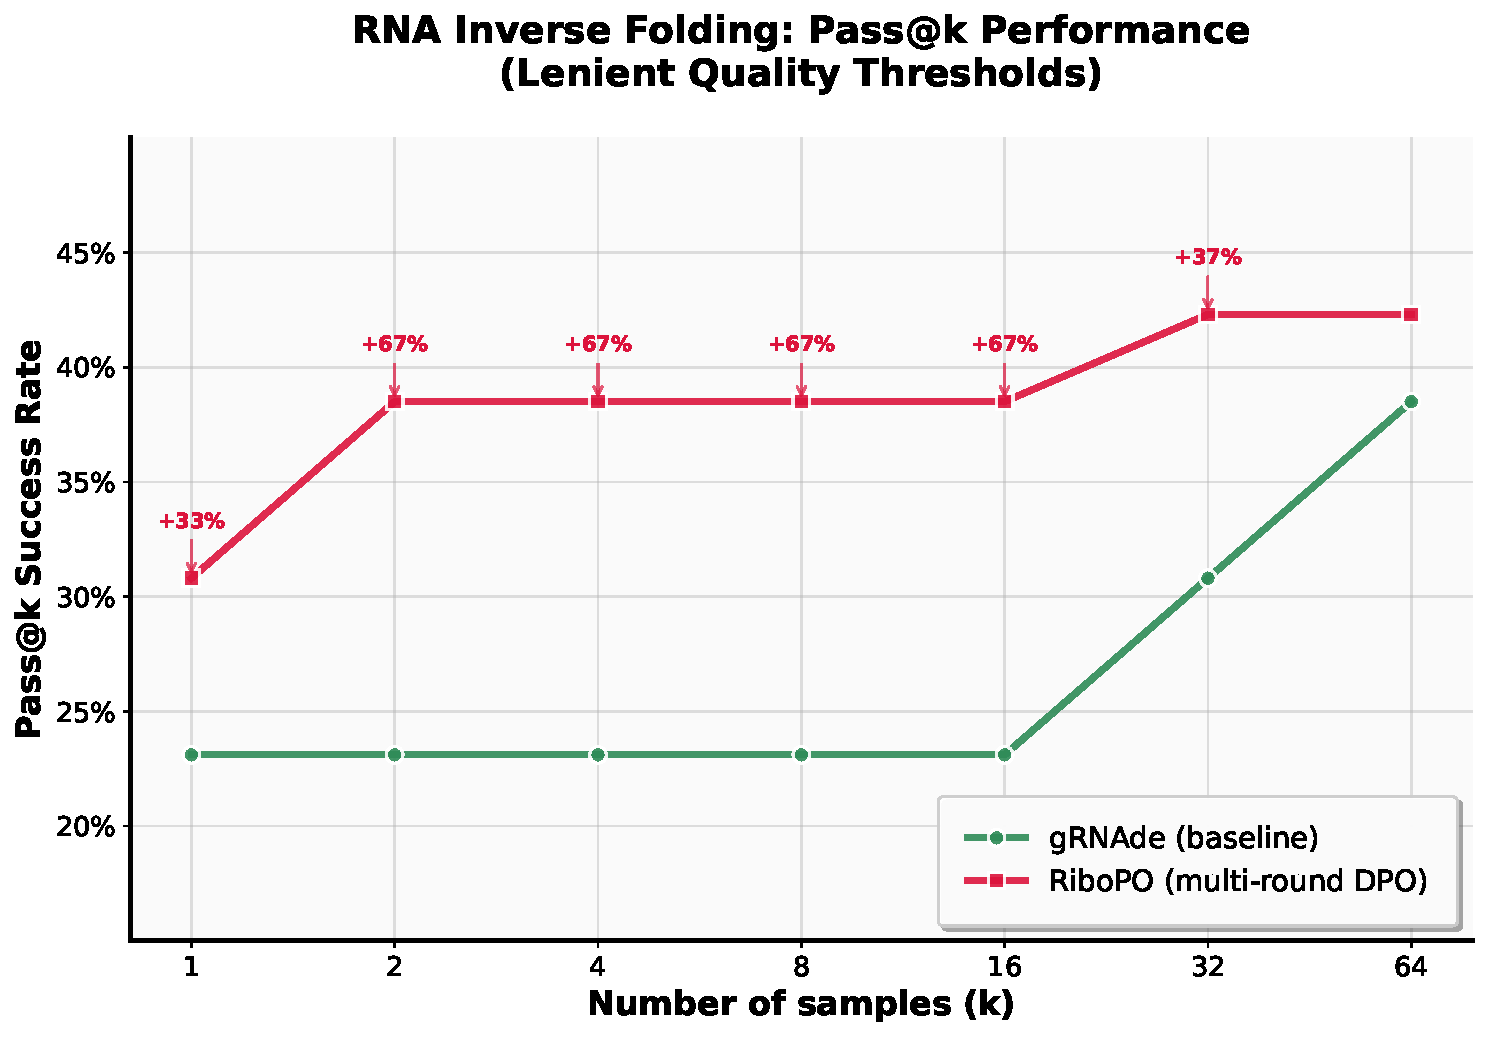
\includegraphics[width=\columnwidth]{figs/pass_at_k_publication.pdf}
%   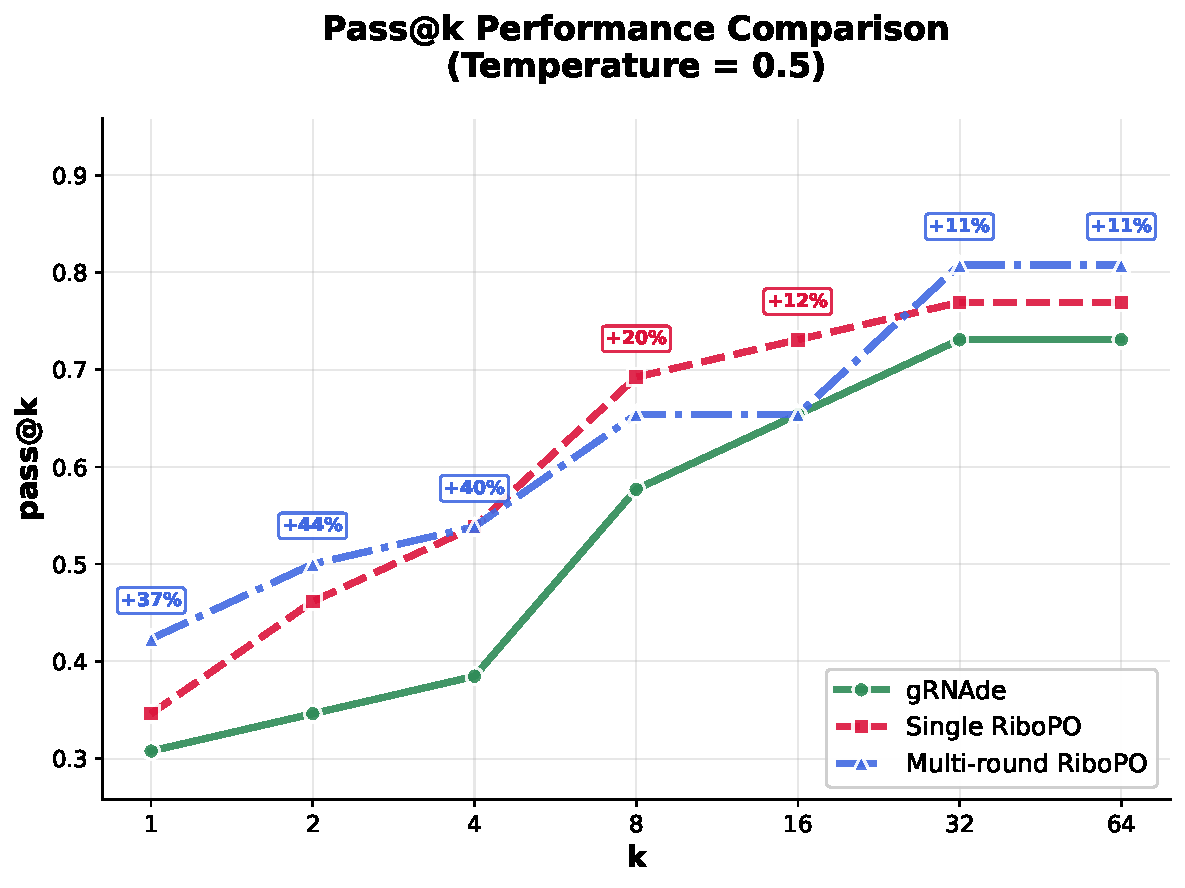
\includegraphics[scale=0.3]{figs/final_exact_passk_temp0.5.pdf}
%   \vspace{-6pt}
%   \caption{\textbf{Sampling efficiency via pass@k.}
%   RiboPO consistently dominates gRNAde across $k\!\in\!\{1,2,4,8,16,32,64\}$, with the largest gains at small $k$ (screening regime).}
%   \label{fig:passk}
%   \vspace{-6pt}
% \end{figure}


\paragraph{Multi-round DPO drives measurable distribution shifts.}
Figure~\ref{fig:dist_shift} compares gRNAde and RiboPO after multi-round training on TM-score, RMSD, pLDDT, and MFE. We observe that RMSD and MFE distributions move toward higher-quality regions: the incidence of poor outliers (RMSD $>15$\AA, MFE $>-10$ kcal/mol) decreases while the mass of stable, low-energy designs increases (mean MFE $-16.5\rightarrow-18.9$ kcal/mol). pLDDT, already relatively high for the base model (mean $\sim 0.62$), becomes more stable with enrichment in the 0.65–0.8 range and suppression of low-confidence cases. TM-score exhibits a “center-convergence” pattern: scores at the low end are lifted, yet samples concentrate near the middle (0.15–0.40), consistent with indirect optimization via RMSD and pLDDT rather than TM-score itself. From the RL viewpoint, these shifts confirm that large early margins ($\gamma_r$ high) promote coarse exploration and smaller later margins refine toward explicitly rewarded regions (RMSD, MFE). From the RNA viewpoint, the policy first secures gross foldability and energetic feasibility, then favors finer conformational improvements; \textbf{this two-phase process mirrors natural RNA evolution}.
% 这部分我觉得没啥改的


% ==============================================================================
% FIGURE 2: COMBINED ANALYSIS (Pass@k and Distributions)
% ==============================================================================
\begin{figure*}[t!]
\centering

% --- Left Subfigure: Pass@k Curve ---
\begin{subfigure}[b]{0.48\textwidth}
\centering
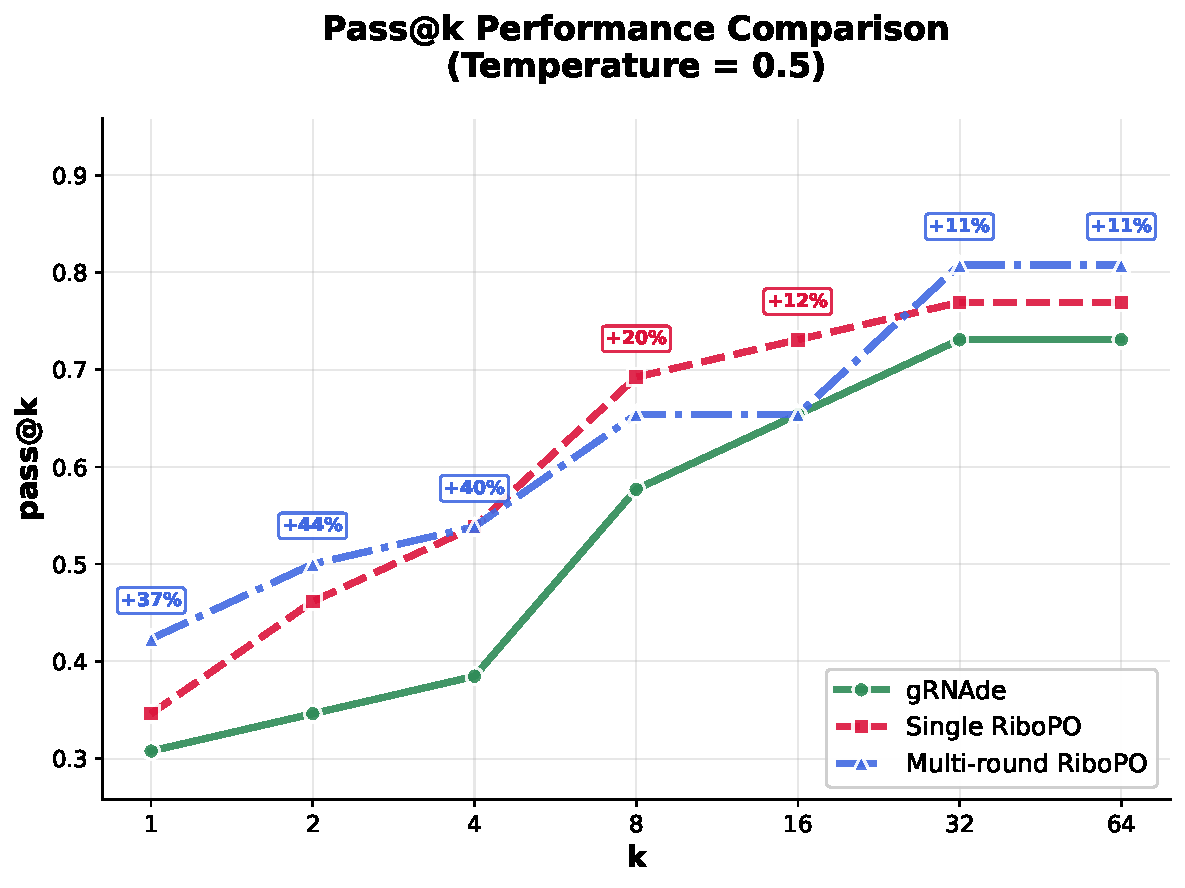
\includegraphics[width=\textwidth]{figs/final_exact_passk_temp0.5.pdf}
\caption{Pass@k Sampling Efficiency}
\label{fig:passk_curve}
\end{subfigure}
% \hfill % This adds a flexible space between the two subfigures
\hspace{0.02cm}
% --- Right Subfigure: Distribution Shifts ---
\begin{subfigure}[b]{0.48\textwidth}
\centering
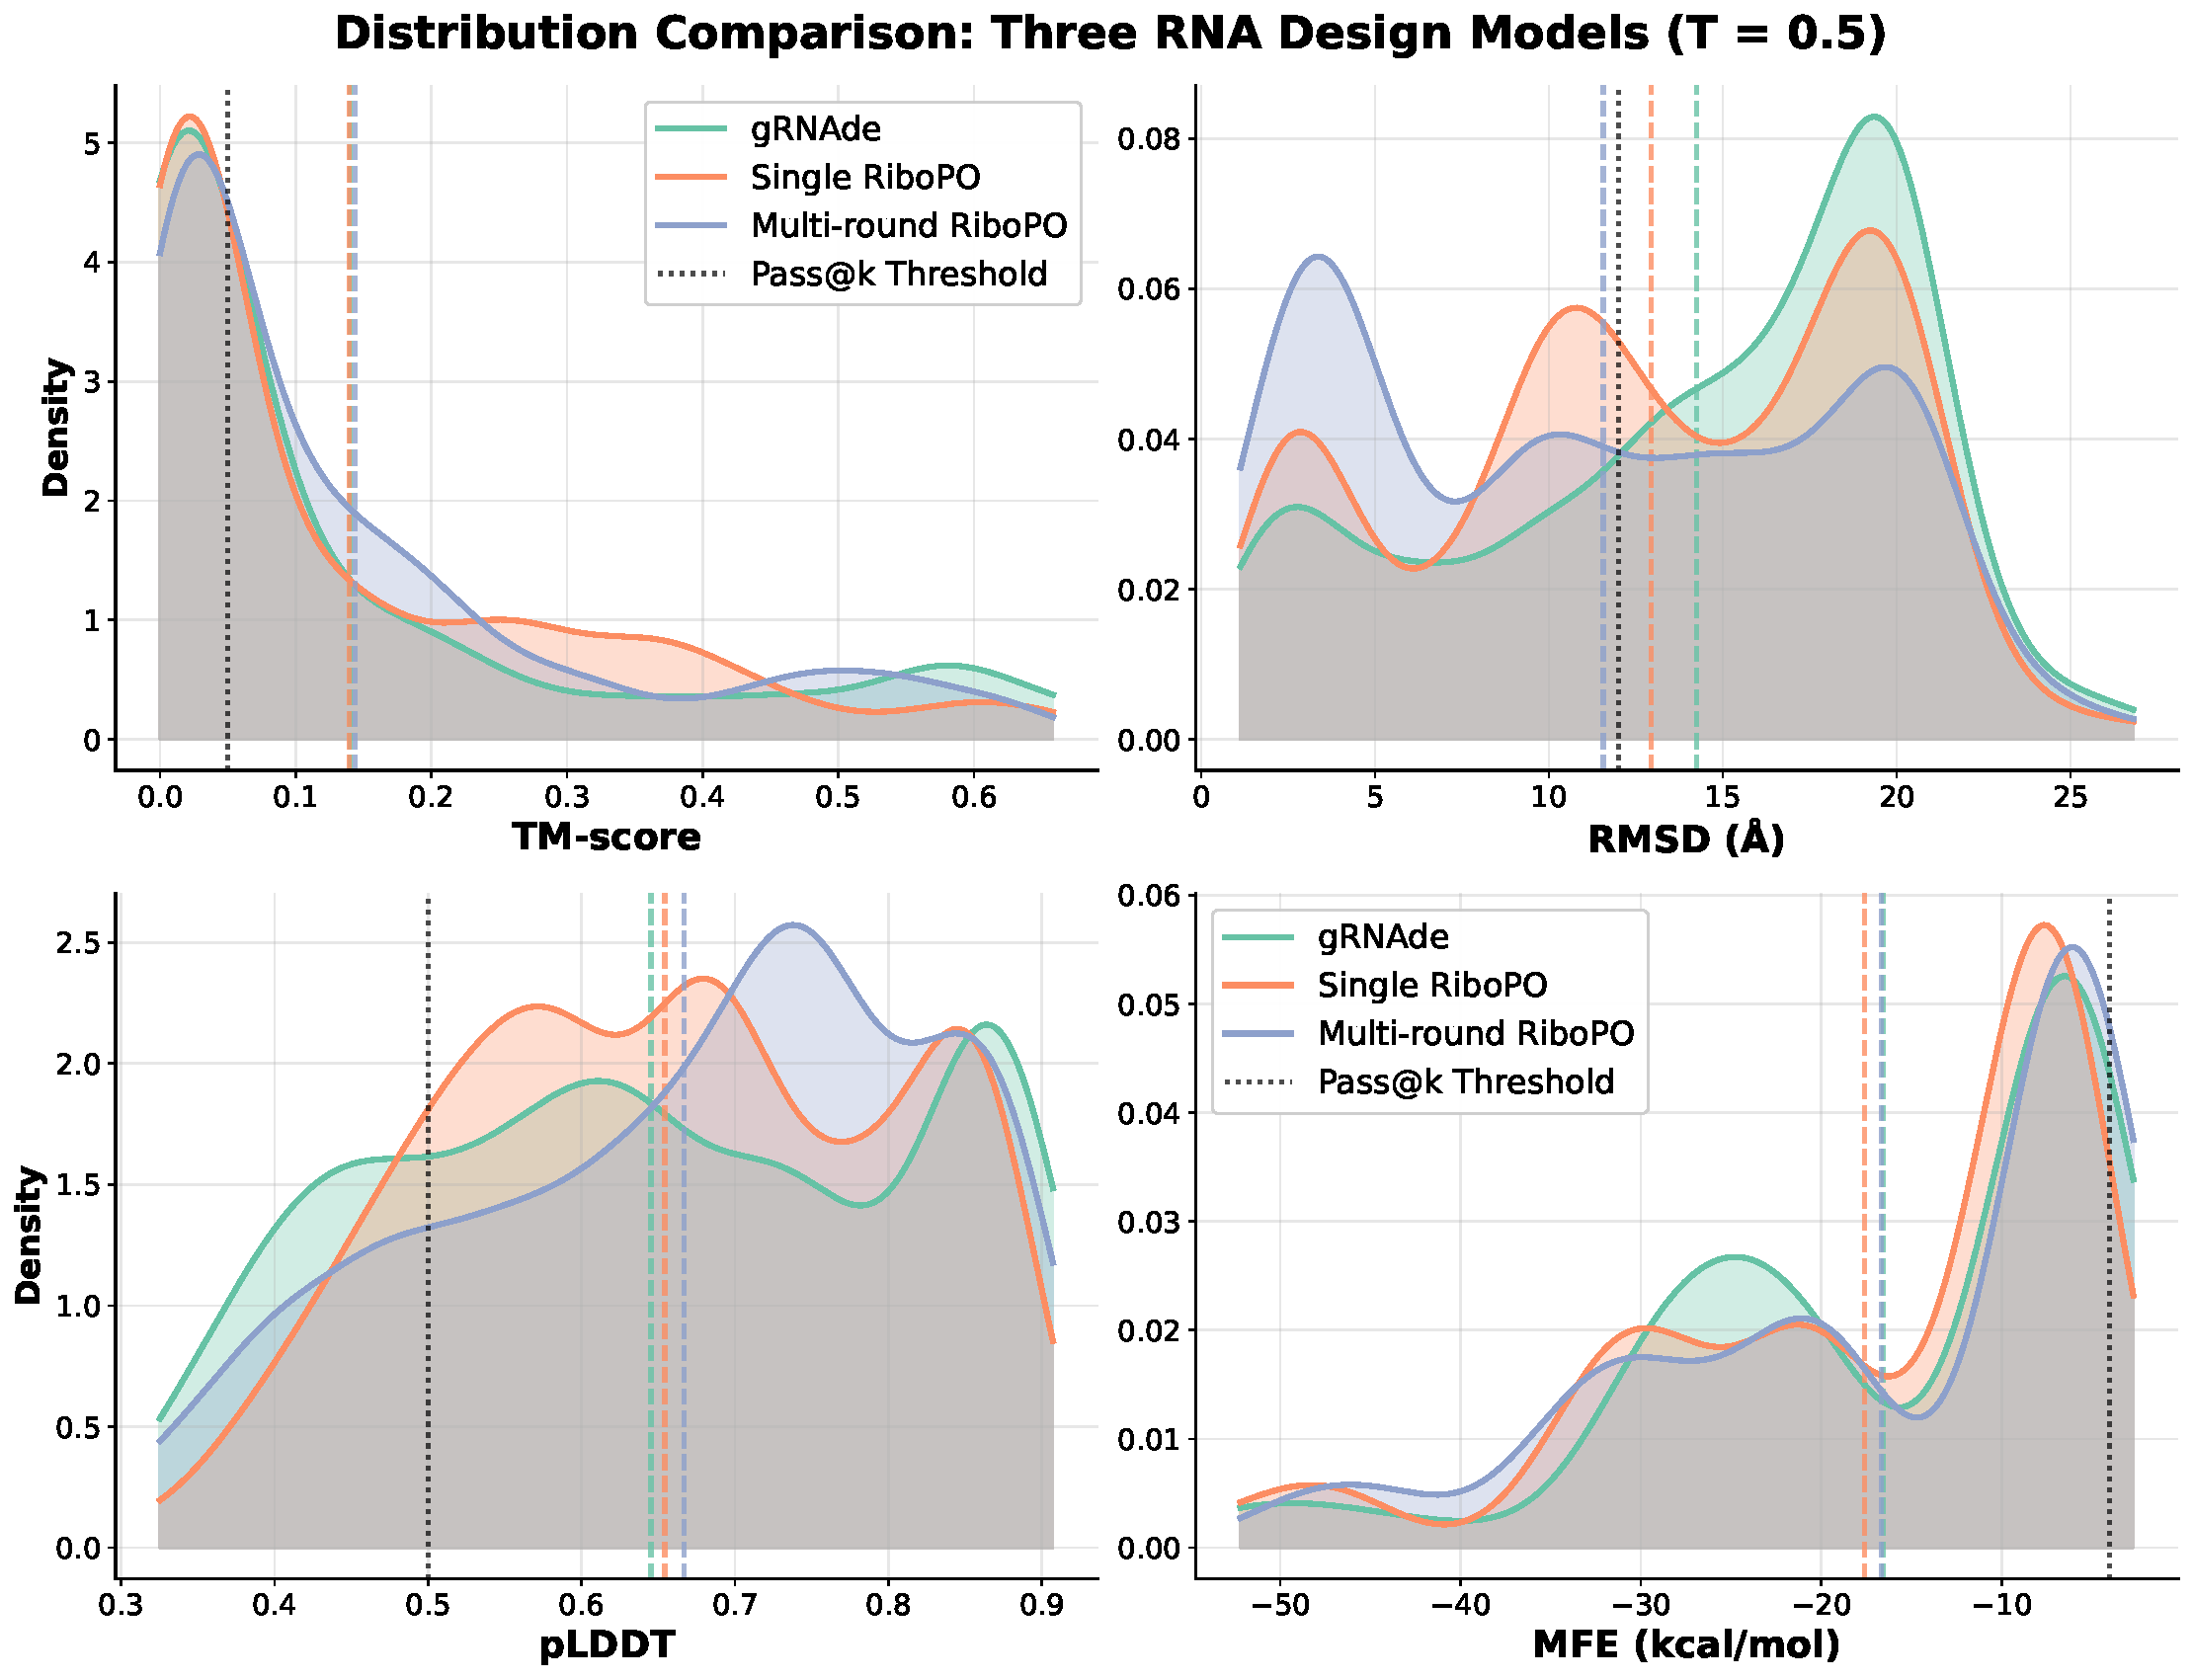
\includegraphics[width=\textwidth]{figs/final_exact_distributions_temp0.5.pdf}
\caption{Metric Distribution Shifts}
\label{fig:dist_shift}
\end{subfigure}

\vspace{-6pt}
\caption{
\textbf{RiboPO improves both sampling efficiency and the quality distribution of generated sequences.}
\textbf{(a)} Pass@k performance shows RiboPO consistently dominates gRNAde across all sample sizes $k$, with the largest gains at the small-$k$ screening regime crucial for practical applications.
\textbf{(b)} Kernel density estimates for key metrics on 14 held-out RNA structures. Multi-round RiboPO shifts the distributions for RMSD and MFE towards more favorable values (indicated by vertical lines) compared to the gRNAde baseline, demonstrating improved designability and thermostability.
}
\label{fig:combined_analysis}
\vspace{-6pt}
\end{figure*}


% \begin{table}[h]
% \centering
% \caption{Pass@k results for generating a sequence with RMSD $< 12$ \AA, pLDDT $> 0.50$, TM-score $> 0.05$, and MFE $< -4.0$ kcal/mol (T = 0.5). RiboPO demonstrates superior sampling efficiency with Multi-round RiboPO achieving the best
% performance.}
% \label{tab:pass_at_k}
% \resizebox{\columnwidth}{!}{%
% \begin{tabular}{lccccccc}
% \toprule
% \textbf{Model} & \textbf{pass@1} & \textbf{pass@2} & \textbf{pass@4} & \textbf{pass@8} & \textbf{pass@16} & \textbf{pass@32} & \textbf{pass@64} \\
% \midrule
% gRNAde & 0.308 & 0.346 & 0.385 & 0.577 & 0.654 & 0.731 & 0.731 \\
% RiboPO (Round 1) & 0.346 & 0.462 & 0.538 & \textbf{0.692} & \textbf{0.731} & 0.769 & 0.769 \\
% RiboPO (Round 4) & \textbf{0.423} & \textbf{0.500} & \textbf{0.538} & 0.654 & 0.654 & \textbf{0.808} & \textbf{0.808} \\
% \bottomrule
% \end{tabular}}
% \end{table}

\begin{table}[!t]
\centering
\caption{Pass@k results for generating a sequence with RMSD $< 12$ \AA, pLDDT $> 0.50$, TM-score $> 0.05$, and MFE $< -4.0$ kcal/mol (T = 0.5). RiboPO demonstrates superior sampling efficiency with Multi-round RiboPO achieving the best performance.}
\label{tab:pass_at_k}
\resizebox{\columnwidth}{!}{%
\begin{tabular}{lccccccc}
\toprule
\textbf{Model} & \textbf{pass@1} & \textbf{pass@2} & \textbf{pass@4} & \textbf{pass@8} & \textbf{pass@16} & \textbf{pass@32} & \textbf{pass@64} \\
\midrule
gRNAde & 0.308 & 0.346 & 0.385 & 0.577 & 0.654 & 0.731 & 0.731 \\
RiboPO (Round 1) & 0.346 & 0.462 & 0.538 & \textbf{0.692} & \textbf{0.731} & 0.769 & 0.769 \\
RiboPO (Round 4) & \textbf{0.423} & \textbf{0.500} & \textbf{0.538} & 0.654 & 0.654 & \textbf{0.808} & \textbf{0.808} \\
\bottomrule
\end{tabular}}
\end{table}



\subsection{Ablation Studies}
\label{subsec:ablation_studies}

\paragraph{Ablation on loss components and hyperparameters.}
To test whether our loss formulation truly supports multi-objective optimization, we ablate both loss components and loss weights (Table~\ref{tab:ablation_loss}). Removing the DPO term ($\beta{=}0$) causes broad degradation in structural metrics (pLDDT $0.62$, RMSD $11.50$), confirming that pairwise preference learning is the main driver of structural improvements. Ablating the SFT term ($\lambda_{\text{SFT}}{=}0$) increases diversity ($0.93$) and makes MFE more negative ($-42.60$~kcal/mol), but markedly worsens tertiary quality (TM-score $0.19$, RMSD $13.55$). This indicates that SFT functions as a distributional anchor that prevents over-exploitation of low-energy but geometrically unrealistic regions; \textbf{removing SFT trades stability for 3D realism}. 

Loss-weight ablation further shows a clear trade-off governed by $\beta$. 
{
According to the DPO objective, 
a larger $\beta$ weakens the KL regularization against the reference policy $\pi_{ref}$, allowing the model to deviate more aggressively toward aligning with the chosen responses. Conversely, smaller $\beta$ values enforce a stronger trust region around $\pi_{ref}$. The detailed theoretical analysis is at Appendix \ref{app:theory}.
}
Consequently, the setting $\beta=0.12$ achieves highly optimized performance across most evaluation metrics. By contrast, $\beta=0.5$ yields slightly better performance than $\beta=1.0$, reflecting a more balanced optimization between fidelity to $\pi_{ref}$ and adaptation to preferences. In the case of MFE, the performance exhibits an inverse relationship with $\beta$: larger values consistently result in superior outcomes. We attribute this to the construction of the pairwise preference data, which introduces no explicit margin for MFE, thereby weakening the available learning signal. In contrast, pLDDT and RMSD provide stronger and more discriminative gradients that dominate optimization when $\beta$ is small, leading to poorer MFE. At smaller $\beta$ values, the stronger KL regularization keeps the policy closer to $\pi_{ref}$ while preference updates are dominated by structural margins, which limits how much MFE can improve. As $\beta$ increases and the KL term weakens, the model can deviate further from $\pi_{ref}$ and better exploit whatever signal about thermodynamic stability is present in the preferences, so MFE benefits disproportionately even though other structural metrics may plateau or decline. These observations highlight that the distribution of the preference dataset plays a pivotal role in shaping DPO performance, which is consistent with recent findings in \citep{Pan2025WhatMI}.


% Loss-weight ablation further shows a clear trade-off governed by $\beta$. Extremely small or large $\beta$ harms tertiary structure (e.g., RMSD $13.39$ at $\beta{=}0.01$ and $13.90$ at $\beta{=}1.0$), while an intermediate $\beta{=}0.12$ achieves the best structural balance (scMCC $0.71$, pLDDT $0.66$, RMSD $10.40$, TM-score $0.30$) with high diversity ($0.90$). Conversely, larger $\beta$ values ($0.5$–$1.0$) yield the most negative MFE ($-42.97$, $-42.61$) but at the cost of 3D fidelity. \textbf{Thus $\beta$ controls the stability–structure trade-off: moderate values optimize structure; large values push toward lower energy.} Sequence-level metrics vary less across $\beta$, suggesting that diversity and recovery are comparatively robust to the preference strength.

% \begin{table}[ht!]
\begin{table}[!t]
\centering
\caption{Ablation study on loss components for single round training}
\label{tab:ablation_loss}
\resizebox{\columnwidth}{!}{%
\begin{tabular}{lccccccccc}
\toprule
\multirow{2}{*}{\textbf{Configuration}} 
& \multicolumn{2}{c}{\cellcolor{blue!10}\textbf{S (Sequence)}} 
& \multicolumn{1}{c}{\cellcolor{blue!10}\textbf{S (2D Struct.)}} 
& \multicolumn{5}{c}{\cellcolor{blue!10}\textbf{T (3D Struct.)}} 
& \multicolumn{1}{c}{\cellcolor{blue!10}\textbf{T (Thermo.)}} \\
\cmidrule(lr){2-3} \cmidrule(lr){4-4} \cmidrule(lr){5-9} \cmidrule(lr){10-10}
& \makecell{Rec.\\ ($\uparrow$)} & \makecell{Div.\\($\uparrow$)} & \makecell{scMCC\\($\uparrow$)} & \makecell{pLDDT\\($\uparrow$)} & \makecell{\%pLDDT\\$\geq$0.70} & \makecell{RMSD\\($\downarrow$)} & \makecell{\%RMSD\\$\leq 8\,\text{\AA}$} & \makecell{TM-sc.\\($\uparrow$)} & \makecell{MFE\\($\downarrow$)} \\
\midrule
w/o $\mathcal{L}_{\mathrm{DPO}}$ ($\beta=0$) & 0.49 & 0.85 & 0.61 & 0.62 & 0.36 & 11.50 & 0.36 & 0.27 & -33.68 \\
w/o $\mathcal{L}_{\mathrm{SFT}}$ ($\lambda_{SFT}=0$) & 0.44 & 0.93 & 0.64 & 0.62 & 0.42 & 13.55 & 0.39 & 0.19 & \textbf{-42.60} \\
\midrule
% RiboPO ($\beta=0.01$) & 0.46 & 0.87 & 0.59 & 0.59 & 0.28 & 13.39 & 0.37 & 0.21  & -41.38 \\
RiboPO ($\beta=0.5$) & 0.47 & 0.88 & 0.57 & 0.62 & 0.40 & 11.96 & 0.45 & 0.25 & -41.05 \\
RiboPO ($\beta=1.0$) & 0.49 & 0.85 & 0.59 & 0.60 & 0.35 & 13.90 & 0.26 & 0.20 & -41.86 \\
\midrule
RiboPO ($\beta=0.12$) & \textbf{0.50} & \textbf{0.90} & \textbf{0.71} & \textbf{0.66} & \textbf{0.45} & \textbf{10.40} & \textbf{0.45} & \textbf{0.30} & -35.83 \\
\bottomrule
\end{tabular}%
}
\end{table}

\paragraph{Ablation on offline RL algorithms.}
We compare SimPO and DPO under a single round (Table~\ref{tab:ablation_algo}). DPO consistently outperforms SimPO on structural fidelity (scMCC $0.71$ vs.\ $0.66$, RMSD $10.40$ vs.\ $11.36$, TM-score $0.30$ vs.\ $0.27$) and on robustness thresholds (\%RMSD$\leq$8\AA: $0.45$ vs.\ $0.40$; \%pLDDT$\geq 0.70$: $0.45$ vs.\ $0.44$), while maintaining higher diversity ($0.90$ vs.\ $0.87$). SimPO shows slightly higher recovery ($0.51$ vs.\ $0.50$) and more negative MFE ($-36.28$ vs.\ $-35.83$). These results suggest that DPO’s likelihood-ratio objective with an explicit reference anchor is better at preserving global 3D realism while still exploring diverse sequences; \textbf{SimPO favors stability and exact-token matching slightly more, but at the expense of tertiary structure}.

\begin{table}[t]
\centering
\caption{Comparison of different RL algorithms (DPO and SimPO) with only a single round. DPO demonstrates superior performance across key metrics.}
\label{tab:ablation_algo}
\resizebox{\columnwidth}{!}{%
\begin{tabular}{lccccccccc}
\toprule
\multirow{2}{*}{\textbf{Algorithm}} 
& \multicolumn{2}{c}{\cellcolor{blue!10}\textbf{S (Sequence)}} 
& \multicolumn{1}{c}{\cellcolor{blue!10}\textbf{S (2D Struct.)}} 
& \multicolumn{5}{c}{\cellcolor{blue!10}\textbf{T (3D Struct.)}} 
& \multicolumn{1}{c}{\cellcolor{blue!10}\textbf{T (Thermo.)}} \\
\cmidrule(lr){2-3} \cmidrule(lr){4-4} \cmidrule(lr){5-9} \cmidrule(lr){10-10}
& \makecell{Rec.\\ ($\uparrow$)} & \makecell{Div.\\($\uparrow$)} & \makecell{scMCC\\($\uparrow$)} & \makecell{pLDDT\\($\uparrow$)} & \makecell{\%pLDDT\\$\geq$0.70} & \makecell{RMSD\\($\downarrow$)} & \makecell{\%RMSD\\$\leq$8\AA} & \makecell{TM-sc.\\($\uparrow$)} & \makecell{MFE\\($\downarrow$)} \\
\midrule
SimPO & \textbf{0.51} & 0.87 & 0.66 & 0.65 & 0.44 & 11.36 & 0.40 & 0.27 & \textbf{-36.28} \\
DPO & 0.50 & \textbf{0.90} & \textbf{0.71} & \textbf{0.66} & \textbf{0.45} & \textbf{10.40} & \textbf{0.45} & \textbf{0.30} & -35.83 \\
\bottomrule
\end{tabular}%
}
\end{table}

\paragraph{Analysis of multi-round training strategy.}
Table~\ref{tab:ablation_multiround} disentangles three design choices: curriculum on the preference margin (CL), reference-model updates across rounds, and algorithm family. Multi-round DPO without curriculum already improves over the base, but exhibits moderate RMSD ($13.39$) and limited high-confidence structures (\%pLDDT$\geq 0.70{=}0.39$). Introducing a curriculum that narrows the margin across rounds (\emph{Multi-Round CL DPO}) yields the strongest overall structural performance (scMCC $0.72$, pLDDT $0.65$, RMSD $10.42$, \%RMSD$\leq 8$\AA\ $0.44$, TM-score $0.29$) with good diversity ($0.89$). This aligns with our design: early coarse margins de-noise preferences; later fine margins admit subtle yet consistent improvements, steering the policy into near-native basins. 

Updating the reference model each round dramatically pushes MFE downward ($-48.07$~kcal/mol) but harms structure (RMSD $14.30$, TM-score $0.16$). The moving reference weakens the trust-region effect and effectively “ratchets” the policy toward low-energy pockets even when geometry degrades, indicating reward hacking on stability proxies. A curriculum with SimPO across rounds also achieves very low MFE yet lags on structure, reinforcing that the objective form and anchoring are critical. \textbf{The best balance arises from \emph{fixed-reference} multi-round DPO with a margin curriculum}, which preserves 3D fidelity while improving stability.
% 这个根据新实验结果写点东西就好

\begin{table}[t]
\centering
\caption{Ablation study on multi-round training components. Updating the reference model and using a curriculum for the preference margin are both beneficial. MR: Multi-Round; CL: Curriculum Learning, with narrowing preference margin; Take the checkpoint evaluation results at the end of final iteration.}
\label{tab:ablation_multiround}
\resizebox{\columnwidth}{!}{%
\begin{tabular}{lccccccccc}
\toprule
\multirow{2}{*}{\textbf{Strategy}} 
& \multicolumn{2}{c}{\cellcolor{blue!10}\textbf{S (Sequence)}} 
& \multicolumn{1}{c}{\cellcolor{blue!10}\textbf{S (2D Struct.)}} 
& \multicolumn{5}{c}{\cellcolor{blue!10}\textbf{T (3D Struct.)}} 
& \multicolumn{1}{c}{\cellcolor{blue!10}\textbf{T (Thermo.)}} \\
\cmidrule(lr){2-3} \cmidrule(lr){4-4} \cmidrule(lr){5-9} \cmidrule(lr){10-10}
& \makecell{Rec.\\ ($\uparrow$)} & \makecell{Div.\\($\uparrow$)} & \makecell{scMCC\\($\uparrow$)} & \makecell{pLDDT\\($\uparrow$)} & \makecell{\%pLDDT\\$\geq$0.70} & \makecell{RMSD\\($\downarrow$)} & \makecell{\%RMSD\\$\leq$8\AA} & \makecell{TM-sc.\\($\uparrow$)} & \makecell{MFE\\($\downarrow$)} \\
\midrule
Multi-Round DPO, w/o CL & 0.49 & \textbf{0.91} & 0.69 & 0.64 &  0.39 & 13.39  & 0.39 & 0.24 & -35.10 \\
Reference Model Update & 0.47 & 0.85 & 0.63 & 0.60 & 0.35 & 14.30 & 0.17 & 0.16 & -48.07 \\
Multi-Round CL SimPO & 0.46 & 0.87 & 0.61 & 0.58 & 0.25 & 13.14 & 0.32 & 0.21 & \textbf{-48.22} \\
Multi-Round CL DPO & \textbf{0.51} & 0.89 & \textbf{0.72} & \textbf{0.65} & \textbf{0.42} & \textbf{10.42} & \textbf{0.44} & \textbf{0.29} & -35.22 \\
\bottomrule
\end{tabular}%
}
\end{table}


% \subsection{Case study} % 4.4, Figure 2, table 4
% \label{subsec:case_study}

% To provide a qualitative understanding of RiboPO's improvements, we present a case study on the [PDB ID, e.g., 5A2Q] backbone in Figure~\ref{fig:case_study}. While the baseline model generates a sequence that folds with reasonable 3D accuracy, our RiboPO-designed sequence achieves a significantly more favorable MFE, indicating a more stable and likely more functional structure.


\subsection{Transfer to a Second Base Model}
\label{subsec:rifold_transfer_main}

A central concern for any "general framework" claim is whether the recipe transfers to architecturally different base models. We apply RiboPO to RiFold \citep{liu2025sentences}, a stochastic-order autoregressive GNN trained with masked language modeling that is architecturally and inductively distinct from gRNAde. Using the same DPO loss, the same preference filter, and identical $\beta = 0.12$ and $\lambda_{\text{SFT}}$, we adapt only the learning rate ($1\!\times\!10^{-5}$ for the off-policy RiFold setting vs.\ $1.8\!\times\!10^{-4}$ for gRNAde). Conservative-setting RiFold + RiboPO improves Vienna MFE by $+14\%$ ($-23.39 \to -26.61$ kcal/mol) with $+0.8\%$ scMCC and a small GC shift ($+0.065$). The aggressive setting illustrates the diagnostic value of SSTT: $+31\%$ MFE comes with GC drift of $+0.185$, exactly the compositional reward-hacking signature predicted by Section~\ref{subsubsec:heteroscedastic} --- a failure that single-axis MFE evaluation would miss. Full results and hyperparameter sweep in Appendix~\ref{app:rifold_transfer}; the gRNAde main result (where GC \emph{decreases}) remains the cleanest evidence of genuine, non-compositional optimization.


\subsection{GC-Controlled Thermodynamic Surplus}
\label{subsec:gc_control_main}

The reviewer-relevant question for any MFE-based reward is: how much of the gain is genuine thermodynamic optimization, and how much is GC enrichment? We answer this directly via a regression analysis on $n=784$ candidate sequences (Appendix~\ref{subsec:gc_control}). Fitting $\widehat{\mathrm{MFE}} = a + b\cdot L + c\cdot(\mathrm{GC}\!\cdot\! L)$ on the gRNAde candidate pool, RiboPO sequences exhibit a residual MFE of $-2.48$ kcal/mol after removing the length- and GC-driven component (paired Wilcoxon $p = 1.3\!\times\!10^{-7}$, $71/98$ targets favor RiboPO). The total mean $\Delta\mathrm{MFE}$ is $-3.57$ kcal/mol, of which only $-1.09$ kcal/mol ($31\%$) is explained by the small GC shift ($0.595\!\to\!0.608$, $+0.013$); the GC-independent component is $-2.48$ kcal/mol ($69\%$). Cross-engine consistency (Vienna $\leftrightarrow$ NUPACK $\leftrightarrow$ RNAstructure, Spearman $\rho \in [0.95, 0.99]$ on per-target $\Delta\mathrm{MFE}$) further rules out reward hacking on the training-time predictor.


\subsection{Statistical Robustness across 21 Metrics}
\label{subsec:robustness_main}

We aggregate four data sources (4-seed re-evaluations on $98$ targets, per-target thermodynamic battery, joint pass@k, per-residue motif data) into a unified panel of 21 metrics (Appendix~\ref{app:robustness_panel}). Of these, $20$ improve in the favorable direction and $17$ are statistically significant at $p < 0.05$. The headline new results, all on the full $98$-structure DAS test set:

\begin{itemize}[leftmargin=1.5em,itemsep=2pt,topsep=2pt]
\item \textbf{Target-structure probability $P(S_0)$:} $0.0027 \to 0.0215$, $+687\%$ ($p = 1.6\!\times\!10^{-5}$, Cohen's $d_z = 25.7$). RiboPO sequences are $\sim 8\!\times$ more likely to actually fold to the target structure under the partition function.
\item \textbf{Designability rates:} RMSD$<$8\AA\ from $0.425 \to 0.490$ ($+15.3\%$, $p = 4.4\!\times\!10^{-3}$); pLDDT$\geq$0.70 from $0.386 \to 0.448$ ($+16.0\%$, $p = 6.5\!\times\!10^{-3}$).
\item \textbf{Joint-criterion sample efficiency:} under $C_1 := \{\text{pLDDT}\geq 0.70 \wedge \text{RMSD}\leq 8\,\text{\AA}\}$, RiboPO pass@1 is $0.258$ vs.\ gRNAde pass@64 $= 0.154$ --- a $\boldsymbol{64\times}$ \textbf{sample-efficiency gain} corresponding to $\sim$97\% reduction in downstream folding cost per validated design.
\item \textbf{Functional contacts:} INF--Watson-Crick $+51.5\%$ ($p = 7.6\!\times\!10^{-3}$), INF--Non-canonical (A-minor / ribose zipper / sheared GA contacts) $+23.6\%$ ($p = 9.6\!\times\!10^{-4}$). Despite the $-5.3\%$ recovery decrease, functional contacts measured by INF \emph{improve}.
\item \textbf{Melting temperature:} $36.30 \to 37.51\,^\circ$C ($+1.2\,^\circ$C, $p = 2.4\!\times\!10^{-2}$).
\end{itemize}

\paragraph{Honest disclosure.}
The 3D RhoFold+ aggregate metrics (scTM, scGDT, scRMSD) improve directionally but are not statistically significant at the per-structure level ($46$--$56$ out of $98$ targets favor RiboPO). This is consistent with RhoFold+ predictions having large per-target variance that dominates the gain on individual targets. The strongest evidence in the panel is in the thermodynamic and 2D axes (per-target Wilcoxon at $p < 0.005$ on $63$--$72$ of $98$ targets); we report the 3D limitations transparently rather than relying on more optimistic 4-seed numbers. We additionally observe that on short sequences ($\leq 58$ nt), MFE actually slightly regresses ($+2.15$ kcal/mol on $n=27$ targets) while $P(S_0)$ and ED still improve --- on short sequences, RiboPO trades MFE for specificity, an adaptive (not uniform) optimization profile worth flagging for downstream applications.

